\documentclass[12pt, letterpaper]{article}
\usepackage[margin=0.5in]{geometry}
\usepackage{amsmath}
\usepackage{amssymb}
\usepackage{pgfplots}
\pgfplotsset{compat=newest}
\usetikzlibrary{intersections}
\usepackage{tkz-euclide}
\usepackage[labelfont={footnotesize,it,bf},textfont={small,it}]{caption}

%% \usepackage{fancyhdr}
%% \usepackage{fancybox,framed}
\usepackage{fancybox}

\pgfplotsset{
  standard/.style = thick,
  trig format=rad,
  enlargelimits,
  axis line style={latex-latex},
  axis x line=middle,
  axis y line=middle,
  enlarge x limits=0.15,
  enlarge y limits=0.15,
  every axis x label/.style={at={(current axis.right of origin)}, anchor=north west},
  every axis y label/.style={at={(current axis.above origin)}, anchor=south east},
  grid=both,
  ticklabel style={font=\tiny,fill=white},
}

\title{Assignment 0}
\author{Lokesh Mohanty (SR no: 21014)}
\date{August 2022}

%% \pagestyle{fancy}

%% \renewcommand{\headrulewidth}{0pt}
%% \renewcommand{\footrulewidth}{0pt}

%% \fancyhf{}
%% \rhead{
%%   Lokesh Mohanty\\
%%   SR No: 21014\\
%%   Section 1
%% }
%% \rfoot{Page \thepage}

\newcommand{\M}{\mathbb{M}^{2x2}}

\begin{document}

\maketitle

\textbf{Why do you want to join this course?}\\
I know the basics of linear algebra. I want to take this course to learn to use features of linear algebra computationally as it is a necessity for data science and since I am from CDS, it's a basic requirement for any research that I do.

%% -------------------------------- Problem #1 -----------------------------------------------

\paragraph{1.} \textbf{Vector Space}\\\\
Verify if the following form a vector space.

%% -------------------------------- Problem #1.a -----------------------------------------------
\subparagraph{(a)} Given that,
\begin{equation}
  \label{1a}
  \mathbb{V} =
  \left\{
  \begin{pmatrix}w \\ x \\ y \\ z\end{pmatrix} \, \middle| \, w-x-y+z = 0; \, w,x,y,z \in \mathbb{R} 
    \right\}
\end{equation}\\

For $\mathbb{V}$ to be a vector space, it should have atleast one element.\\
Lets consider an element
$\mathbf{v} = \begin{pmatrix}0\\0\\0\\0\end{pmatrix}$ in
$\mathbb{V}$ where w = x = y = z = 0,\\
it satisfies the condition $w - x - y + z = 0$ and $w,x,y,z \in\mathbb{R}$\\
Hence, $\mathbf{v}\in\mathbb{V} \implies \mathbb{V}$ is not empty\\

Let $v_1, v_2, v_3$ be vectors in the set $\mathbb{V}$, then
\begin{equation}
  \label{1a1}
  \begin{split}
    v_1 = \begin{pmatrix}w_1\\x_1\\y_1\\z_1\end{pmatrix}, w_1 - x_1 - y_1 + z_1 = 0\\
    v_2 = \begin{pmatrix}w_2\\x_2\\y_2\\z_2\end{pmatrix}, w_2 - x_2 - y_2 + z_2 = 0\\
    v_3 = \begin{pmatrix}w_3\\x_3\\y_3\\z_3\end{pmatrix}, w_3 - x_3 - y_3 + z_3 = 0
  \end{split}
\end{equation}

\begin{enumerate}

\item \textbf{Closure under addition property}
  ($u + v \in \mathbb{V}, \, \forall \, u, v \in \mathbb{V}$)

\textit{\underline{Proof}:}

  let $ v_1 + v_2 = l$; where $l = \begin{pmatrix}l_1\\l_2\\l_3\\l_4\end{pmatrix}$
  $
  \implies w = \begin{pmatrix}w_1 + w_2\\x_1 + x_2\\y_1 + y_2\\z_1 + z_2\end{pmatrix}
    = \begin{pmatrix}l_1\\l_2\\l_3\\l_4\end{pmatrix}
  $ 

  As per equation~\ref{1a1}, \\
  $w_1 + x_1 + y_1 + z_1 = 0$ and
  $w_2 + x_2 + y_2 + z_2 = 0$
  \[
  \begin{split}
  &\implies (w_1 - x_1 - y_1 + z_1) + (w_2 - x_2 - y_2 + z_2) = 0 \\
  &\implies (w_1 + w_2) - (x_1 + x_2) - (y_1 + y_2) + (z_1 + z_2) = 0\\
  &\implies l_1 - l_2 - l_3 + l_4 = 0
  \end{split}
  \]
  $\implies l = \begin{pmatrix}l_1\\l_2\\l_3\\l_4\end{pmatrix}$ and $l_1 - l_2 - l_3 + l_4 = 0$
  $\implies l \in \mathbb{V}$\\
  $\implies\boxed{v_1 + v_2 \in\mathbb{V}, \, \forall\, v_1,v_2 \in\mathbb{V}}$

\item \textbf{Commutative property}
  ($u + v = v + u, \, \forall \, u, v \in \mathbb{V}$)

\textit{\underline{Proof}:}

  \begin{equation}
  \label{1a2}
  v_1 + v_2 = \begin{pmatrix}w_1 + w_2\\x_1 + x_2\\y_1 + y_2\\z_1 + z_2\end{pmatrix},
  v_2 + v_1 = \begin{pmatrix}w_2 + w_1\\x_2 + x_1\\y_2 + y_1\\z_2 + z_1\end{pmatrix} 
  \end{equation}

  Since the set of $\mathbb{R}$ is commutative under addition,
  \begin{equation}
  \label{1a3}
  \begin{split}
    w_1 + w_2 &= w_2 + w_1,\\
    x_1 + x_2 &= x_2 + x_1,\\
    y_1 + y_2 &= y_2 + y_1,\\
    z_1 + z_2 &= z_2 + z_1,
  \end{split}
  \end{equation}

  $\therefore$ from equation~\ref{1a2} and~\ref{1a3},\,
  $\boxed{v_1 + v_2 = v_2 + v_1}$

\item \textbf{Associative property}
  ($u + (v + w) = (u + v) + w, \, \forall \, u, v \in \mathbb{V}$)

\textit{\underline{Proof}:}

  \begin{equation}
  \label{1a4}
  v_1 + (v_2 + v_3) = \begin{pmatrix}w_1 + (w_2 + w_3)\\x_1 + (x_2 + x_3)\\y_1 + (y_2 + y_3)\\z_1 + (z_2 + z_3)\end{pmatrix},
  (v_1 + v_2) + v_3 = \begin{pmatrix}(w_1 + w_2) + w_3\\(x_1 + x_2) + x_3\\(y_1 + y_2) + y_3\\(z_1 + z_2) + z_3\end{pmatrix},
  \end{equation}

  Since the set of $\mathbb{R}$ is associative under addition,
  \begin{equation}
  \label{1a5}
  \begin{split}
    w_1 + (w_2 + w_3) &= (w_1 + w_2) + w_3,\\
    x_1 + (x_2 + x_3) &= (x_1 + x_2) + x_3,\\
    y_1 + (y_2 + y_3) &= (y_1 + y_2) + y_3,\\
    z_1 + (z_2 + z_3) &= (z_1 + z_2) + z_3,
  \end{split}
  \end{equation}

  $\therefore$ from equation~\ref{1a4} and~\ref{1a5},\,
  $\boxed{v_1 + v_2 = v_2 + v_1}$

\item \textbf{Zero vector}
  ($0 \in \mathbb{V}$, such that $v + 0 = v, \, \forall \, v \in \mathbb{V}$)

\textit{\underline{Proof}:}

  Let Zero vector ($0$) be a vector with all elements as $0$
  \[
   i.e., \,\,\,\, 0 = \begin{pmatrix}0\\0\\0\\0\end{pmatrix},
   \implies  0 - 0 - 0 + 0 = 0
  \]
  Hence as per equation~\ref{1a}, $\boxed{0 \in \mathbb{V}}$
  \[
    v_1 + 0
    = \begin{pmatrix} w_1 + 0\\ x_1 + 0\\ y_1 + 0\\ z_1 + 0 \end{pmatrix}
    = \begin{pmatrix} w_1\\ x_1\\ y_1\\ z_1 \end{pmatrix}
    = v_1
    \implies \boxed{v_1 + 0 = v_1}
  \]

\item \textbf{Additive inverse}
  (Each $v \in \mathbb{V}$ has a $w \in \mathbb{V}$ such that $v + w = 0$)

\textit{\underline{Proof}:}

  Let $\exists \, w$ such that $v + w = 0$
  \[
    \implies w = -v = -\begin{pmatrix}w\\x\\y\\z\end{pmatrix}
    = \begin{pmatrix}-w\\-x\\-y\\-z\end{pmatrix}
  \]
  As per equation~\ref{1a},
  \[(-w) - (-x) - (-y) + (-z) = -(w -x -y +z) = 0\\ \]
  \[\implies w \in \mathbb{V} \]

  \[ \boxed{\therefore \text{there exists an additive inverse in $\mathbb{V}$ for every }v \in \mathbb{V}} \]

\item \textbf{Closure under scalar Multiplication}
  ($cu \in \mathbb{V}, \forall u \in \mathbb{V}$ and $c \in \mathbb{R}$)

\textit{\underline{Proof}:}

  \[
    \forall c \in \mathbb{R} \text{ and } \forall v \in \mathbb{V}, \,\,
    cv = c\begin{pmatrix}w\\x\\y\\z\end{pmatrix}
    = \begin{pmatrix}cw\\cx\\cy\\cz\end{pmatrix}
  \]
  As per equation~\ref{1a},
  \[(cw) - (cx) - (cy) + (cz) = c(w -x -y +z) = 0\\ \]
  \[\implies \boxed{cv \in \mathbb{V}} \]
  Hence $\mathbb{V}$ is closed under scalar multiplication

\item \textbf{Distributive property for scalar addition}
  ((c + d)v = cv + dv, $\forall v \in \mathbb{V}$ and $\forall c,d \in \mathbb{R}$)

\textit{\underline{Proof}:}

  LHS $\to (c + d)v$; RHS $\to cv + dv$;

  Solving LHS:
  \begin{equation}
  \label{1a6}
    (c + d)v
    = (c + d)\begin{pmatrix}w\\x\\y\\z\end{pmatrix}
    = \begin{pmatrix}(c + d)w\\(c + d)x\\(c + d)y\\(c + d)z\end{pmatrix}
    = \begin{pmatrix}cw + dw\\cx + dx\\cy + dy\\cz + dz\end{pmatrix}
  \end{equation}

  Solving RHS:
  \begin{equation}
  \label{1a7}
    cv + dv
    = c\begin{pmatrix}w\\x\\y\\z\end{pmatrix} + d\begin{pmatrix}w\\x\\y\\z\end{pmatrix}
    = \begin{pmatrix}cw\\cx\\cy\\cz\end{pmatrix} + \begin{pmatrix}dw\\dx\\dy\\dz\end{pmatrix}
    = \begin{pmatrix}cw + dw\\cx + dx\\cy + dy\\cz + dz\end{pmatrix}
  \end{equation}

  From equations~\ref{1a6} and~\ref{1a7}, $\boxed{LHS = RHS}$
  \\Hence proved

\item \textbf{Distributive property for vector addition}
  (c(v + w) = cv + cw, $\forall v,w \in \mathbb{V}$ and $\forall c \in \mathbb{R}$)

\textit{\underline{Proof}:}

  LHS $\to c(v_1 + v_2)$; RHS $\to cv_1 + cv_2$;

  Solving LHS:
  \begin{equation}
  \label{1a8}
    c(v_1 + v_2)
    = c\begin{pmatrix}w_1 + w_2\\x_1 + x_2\\y_1 + y_2\\z_1 + z_2\end{pmatrix}
    = \begin{pmatrix}c(w_1 + w_2)\\c(x_1 + x_2)\\c(y_1 + y_2)\\c(z_1 + z_2)\end{pmatrix}
    = \begin{pmatrix}cw_1 + cw_2\\cx_1 + cx_2\\cy_1 + cy_2\\cz_1 + cz_2\end{pmatrix}
  \end{equation}

  Solving RHS:
  \begin{equation}
  \label{1a9}
    cv_1 + cv_2
    = \begin{pmatrix}cw_1\\cx_1\\cy_1\\cz_1\end{pmatrix} + \begin{pmatrix}cw_2\\cx_2\\cy_2\\cz_2\end{pmatrix}
    = \begin{pmatrix}cw_1 + cw_2\\cx_1 + cx_2\\cy_1 + cy_2\\cz_1 + cz_2\end{pmatrix}
  \end{equation}

  From equations~\ref{1a8} and~\ref{1a9}, $\boxed{LHS = RHS}$
  \\Hence proved

\item \textbf{Identity operation}
  (Multiplication by the scalar $1$, such that $1\,v = v, \, \forall \, v \in \mathbb{V}$)

\textit{\underline{Proof}:}

  We know that,
  \begin{equation}
  \label{1a10}
    cv = c\begin{pmatrix}w\\x\\y\\z\end{pmatrix}
    = \begin{pmatrix}cw\\cx\\cy\\cz\end{pmatrix}
  \end{equation}
  \label{1a11}
  Let $c = 1$,
  \begin{equation}
    \implies \begin{pmatrix}cw\\cx\\cy\\cz\end{pmatrix} = \begin{pmatrix}w\\x\\y\\z\end{pmatrix}
  \end{equation}
  Hence as per equations~\ref{1a9} and~\ref{1a10}, $\boxed{1\,v = v, \, \forall \, v \in \mathbb{V}}$

\end{enumerate}

\doublebox{$\therefore$ As $\mathbb{V}$ satisfies all the conditions of a vector space, $\mathbb{V}$ is a vector space.}

%% -------------------------------- Problem #1.b -----------------------------------------------
\subparagraph{(b)} Given that,
\[
  \label{1b}
  \M =
  \left\{
    \begin{pmatrix}a &0\\b &c\end{pmatrix} \, \middle| \, a,b,c \in \mathbb{R} 
  \right\}
\]\\
For $\M$ to be a vector space, it should have atleast one element.\\
Lets consider an element
$\mathbf{m} = \begin{pmatrix}0&0\\0&0\end{pmatrix}$ in
$\M$, where $a = b = c = 0 \implies a,b,c\in\mathbb{R}$\\
Hence, $\mathbf{m}\in\M \implies \M$ is not empty\\

Let $m_1, m_2, m_3$ be matrices in the set $\M$, then
\[
  \label{1b1}
  \begin{split}
    m_1 = \begin{pmatrix}a_1 &0\\b_1 &c_1\end{pmatrix}, \, a_1, b_1, c_1 \in \mathbb{R}\\
    m_2 = \begin{pmatrix}a_2 &0\\b_2 &c_2\end{pmatrix}, \, a_2, b_2, c_2 \in \mathbb{R}\\
    m_3 = \begin{pmatrix}a_3 &0\\b_3 &c_3\end{pmatrix}, \, a_3, b_3, c_3 \in \mathbb{R}\\
  \end{split}
\]

\begin{enumerate}

\item \textbf{Closure under addition property}
  ($u + v \in \M, \, \forall \, u, v \in \M$)

\textit{\underline{Proof}:}

  let $ m_1 + m_2 = l$;
  $\implies m_1 + m_2 = \begin{pmatrix}a_1 + a_2 &0 + 0\\b_1 + b_2 &c_1 + c_2\end{pmatrix} = l$ 

  Since, $\mathbb{R}$ is closed under addition, $a_1 + a_2, b_1 + b_2, c_1+c_2 \in \mathbb{R}$

  $\implies\boxed{m_1 + m_2 \in\M, \, \forall\, m_1,m_2 \in\M}$

\item \textbf{Commutative property}
  ($u + v = v + u, \, \forall \, u, v \in \M$)

\textit{\underline{Proof}:}

  \begin{equation}
  \label{1b2}
  m_1 + m_2 = \begin{pmatrix}a_1 + a_2&0 + 0\\b_1 + b_2&c_1 + c_2\end{pmatrix},
  m_2 + m_1 = \begin{pmatrix}a_2 + a_1&0 + 0\\b_2 + b_1&c_2 + c_1\end{pmatrix} 
  \end{equation}

  Since the set of $\mathbb{R}$ is commutative under addition,
  \begin{equation}
  \label{1b3}
  \begin{split}
    a_1 + a_2 &= a_2 + a_1,\\
    b_1 + b_2 &= b_2 + b_1,\\
    c_1 + c_2 &= c_2 + c_1,
  \end{split}
  \end{equation}

  $\therefore$ from equation~\ref{1b2} and~\ref{1b3},\,
  $\boxed{m_1 + m_2 = m_2 + m_1}$

\item \textbf{Associative property}
  ($u + (v + w) = (u + v) + w, \, \forall \, u, v, w \in \M$)

\textit{\underline{Proof}:}

  \begin{equation}
  \label{1b4}
  \begin{split}
  m_1 + (m_2 + m_3) = \begin{pmatrix}a_1 + (a_2 + a_3)&0 + (0 + 0)\\b_1 + (b_2 + b_3)&c_1 + (c_2 + c_3)\end{pmatrix},\\
  (m_1 + m_2) + m_3 = \begin{pmatrix}(a_1 + a_2) + a_3&(0 + 0) + 0\\(b_1 + b_2) + b_3&(c_1 + c_2) + c_3\end{pmatrix},
  \end{split}
  \end{equation}

  Since the set of $\mathbb{R}$ is associative under addition,
  \begin{equation}
  \label{1b5}
  \begin{split}
    a_1 + (a_2 + a_3) &= (a_1 + a_2) + a_3,\\
    b_1 + (b_2 + b_3) &= (b_1 + b_2) + b_3,\\
    c_1 + (c_2 + c_3) &= (c_1 + c_2) + c_3,
  \end{split}
  \end{equation}

  $\therefore$ from equation~\ref{1b4} and~\ref{1b5},\,
  $\boxed{m_1 + m_2 = m_2 + m_1}$

\item \textbf{Zero matrix}
  ($0 \in \M$, such that $v + 0 = v, \, \forall \, v \in \M$)

\textit{\underline{Proof}:}

  Let Zero vector ($0$) be a vector with all elements as $0$
  \[ i.e., \,\,\,\, 0 = \begin{pmatrix}0&0\\0&0\end{pmatrix} \]
  Hence as per equation~\ref{1b}, $\boxed{0 \in \M}$
  \[
    m_1 + 0
    = \begin{pmatrix} a_1 + 0& 0 + 0\\ b_1 + 0& c_1 + 0 \end{pmatrix}
    = \begin{pmatrix} a_1& 0\\ b_1& c_1 \end{pmatrix}
    = m_1
    \implies \boxed{m_1 + 0 = m_1}
  \]

\item \textbf{Additive inverse}
  (Each $v \in \M$ has a $w \in \M$ such that $v + w = 0$)

\textit{\underline{Proof}:}

  Let $\exists \, w$ such that $m + w = 0$
  \[
    \implies w = -m = -\begin{pmatrix}a&0\\b&c\end{pmatrix}
    = \begin{pmatrix}-a&0\\-b&-c\end{pmatrix}
  \]
  Since $a, b, c \in \mathbb{R} \implies -a, -b, -c \in \mathbb{R} \implies w \in \M$

  \[ \boxed{\therefore \text{there exists an additive inverse in $\M$ for every }v \in \M} \]

\item \textbf{Closure under scalar Multiplication}
  ($cu \in \M, \forall u \in \M$ and $c \in \mathbb{R}$)

\textit{\underline{Proof}:}

  \[
    \forall k \in \mathbb{R} \text{ and } \forall m \in \M, \,\,
    km = k\begin{pmatrix}a&0\\b&c\end{pmatrix}
    = \begin{pmatrix}ka&0\\kb&kc\end{pmatrix}
  \]
  Since $a, b, c \in \mathbb{R} \implies ka, kb, kc \in \mathbb{R} \implies \boxed{km \in \M}$
  \\Hence $\M$ is closed under scalar multiplication

\item \textbf{Distributive property for scalar addition}
  ((c + d)v = cv + dv, $\forall v \in \M$ and $\forall c,d \in \mathbb{R}$)

\textit{\underline{Proof}:}

  LHS $\to (k + l)m$; RHS $\to km + lm$;

  Solving LHS:
  \begin{equation}
  \label{1b6}
    (k + l)m
    = (k + l)\begin{pmatrix}a&0\\b&c\end{pmatrix}
    = \begin{pmatrix}(k + l)a&(k + l)0\\(k + l)b&(k + l)c\end{pmatrix}
    = \begin{pmatrix}ka + la&0\\kb + lb&kc + lc\end{pmatrix}
  \end{equation}

  Solving RHS:
  \begin{equation}
  \label{1b7}
    km + lm
    = k\begin{pmatrix}a&0\\b&c\end{pmatrix} + l\begin{pmatrix}a&0\\b&c\end{pmatrix}
    = \begin{pmatrix}ka&0\\kb&kc\end{pmatrix} + \begin{pmatrix}la&0\\lb&lc\end{pmatrix}
    = \begin{pmatrix}ka + la&0\\kb + lb&kc + lc\end{pmatrix}
  \end{equation}

  From equations~\ref{1b6} and~\ref{1b7}, $\boxed{LHS = RHS}$
  \\Hence proved

\item \textbf{Distributive property for vector addition}
  (c(v + w) = cv + cw, $\forall v,w \in \M$ and $\forall c \in \mathbb{R}$)

\textit{\underline{Proof}:}

  LHS $\to k(m_1 + m_2)$; RHS $\to km_1 + km_2$;

  Solving LHS:
  \begin{equation}
  \label{1b8}
  \begin{split}
    k(m_1 + m_2)
    &= k\begin{pmatrix}a_1 + a_2&0 + 0\\b_1 + b_2&c_1 + c_2\end{pmatrix}\\
    &= \begin{pmatrix}k(a_1 + a_2)&0\\k(b_1 + b_2)&k(c_1 + c_2)\end{pmatrix}\\
    &= \begin{pmatrix}ka_1 + ka_2&0\\kb_1 + kb_2&kc_1 + kc_2\end{pmatrix}
  \end{split}
  \end{equation}

  Solving RHS:
  \begin{equation}
  \label{1b9}
    km_1 + km_2
    = \begin{pmatrix}ka_1&0\\kb_1&kc_1\end{pmatrix} + \begin{pmatrix}ka_2&0\\kb_2&kc_2\end{pmatrix}
    = \begin{pmatrix}ka_1 + ka_2&0\\kb_1 + kb_2&kc_1 + kc_2\end{pmatrix}
  \end{equation}

  From equations~\ref{1b8} and~\ref{1b9}, $\boxed{LHS = RHS}$
  \\Hence proved

\item \textbf{Identity operation}
  (Multiplication by the scalar $1$, such that $1\,v = v, \, \forall \, v \in \M$)

\textit{\underline{Proof}:}

  We know that,
  \begin{equation}
  \label{1b10}
    km = k\begin{pmatrix}a&0\\b&c\end{pmatrix}
    = \begin{pmatrix}ka&0\\kb&kc\end{pmatrix}
  \end{equation}
  \label{1b11}
  Let $k = 1$,
  \begin{equation}
    \implies \begin{pmatrix}ka&0\\kb&kc\end{pmatrix} = \begin{pmatrix}a&0\\b&c\end{pmatrix}
  \end{equation}
  Hence as per equations~\ref{1b9} and~\ref{1b10}, $\boxed{1\,m = m, \, \forall \, m \in \M}$

\end{enumerate}

\doublebox{$\therefore$ As $\M$ satisfies all the conditions of a vector space, $\M$ is a vector space.}

%% -------------------------------- Problem #1.c -----------------------------------------------

\subparagraph{(c)} Given that,
\[
  \label{1c}
  \mathbb{N} = \left\{ f : \mathbb{R} \to \mathbb{R} \, \middle| \, \frac{df}{dx} + 2f = 1 \right\}
\]
For $\mathbb{N}$ to be a vector space, it should have atleast one element.\\
Lets consider an element $g$ such that
$g(x) = \frac{1-e^{-2x}}{2} \implies \frac{dg}{dx} + 2g = 1$\\
Hence, $g \in \mathbb{N} \implies \mathbb{N}$ is not empty\\

Let $f_1, f_2, f_3$ be functions in the set $\mathbb{N}$, then
\begin{equation}
  \label{1c1}
    \frac{df_1}{dx} + 2f_1 = 1, \,
    \frac{df_2}{dx} + 2f_2 = 1
\end{equation}

\begin{enumerate}

\item \textbf{Closure under addition property}
  ($u + v \in \mathbb{N}, \, \forall \, u, v \in \mathbb{N}$)

\textit{\underline{Proof}:}

  \begin{equation}
  \label{1c2}
    \text{let } f_1 + f_2 = g;
    \implies \frac{dg}{dx} = \frac{df_1}{dx} + \frac{df_1}{dx}
  \end{equation}

  Adding equations in~\ref{1c1} and from equation~\ref{1c2},
  \[
  \begin{split}
    &\frac{df_1}{dx} + 2f_1 + \frac{df_2}{dx} + 2f_2 = 1 + 1\\
    \implies &(\frac{df_1}{dx} + \frac{df_2}{dx}) + 2(f_1 + f_2) = 2\\
    \implies &\frac{dg}{dx} + 2g = 2 \neq 1\\
    \implies &g \not\in \mathbb{N}
  \end{split}
  \]
  $\implies\boxed{f_1 + f_2 \not\in\mathbb{N}, \, \forall\, f_1,f_2 \in\mathbb{N}}$

\end{enumerate}

\doublebox{
\begin{minipage}{5.5in}$\therefore$ As $\mathbb{N}$ doesn't satisfy the closure under addition property of a vector space, $\mathbb{N}$ is not a vector space.
\end{minipage}}

%% -------------------------------- Problem #2 -----------------------------------------------
\pagebreak
\paragraph{2.} \textbf{Subspace: }
A non-empty subset $\mathbb{W}$ of a vector space $\mathbb{V}$ over a field $\mathbb{R}$ is a subspace of $\mathbb{V}$ if and only if

\begin{equation}
  \label{2}
  \begin{split}
  &\mathbf{a} \in \mathbb{W}, \mathbf{b} \in \mathbb{W} \implies \mathbf{a} + \mathbf{b} \in \mathbb{W}\\
  &\mathbf{a}\in\mathbb{W}, \alpha \in \mathbb{R} \implies \alpha \mathbf{a}\in\mathbb{W}
  \end{split}
\end{equation}

%% -------------------------------- Problem #2.a -----------------------------------------------
\subparagraph{(a)} Does $\mathbb{V}$ form a subspace of $\mathbb{R}^3$, where
\[
  \mathbb{V} = \left\{\begin{pmatrix}x\\y\\z\end{pmatrix}\middle| \, x,y,z \geq 0\right\}
\]


\begin{enumerate}
  \item $\mathbb{V}$ is not empty as $\begin{pmatrix}0\\0\\0\end{pmatrix}\in\mathbb{V}$
  \item Let $v_1, v_2 \in \mathbb{V}$, such that
  \begin{equation}
    \label{2a}
    \begin{split}
    &v_1 = \begin{pmatrix}x_1\\y_1\\z_1\end{pmatrix},\,
    v_2 = \begin{pmatrix}x_2\\y_2\\z_2\end{pmatrix},\,
    \text{where }x_1,y_1,z_1,x_2,y_2,z_2\geq0\\
    \implies &v_1 + v_2
    = \begin{pmatrix}x_1\\y_1\\z_1\end{pmatrix} +
    \begin{pmatrix}x_2\\y_2\\z_2\end{pmatrix}
    =\begin{pmatrix}x_1 + x_2\\y_1 + y_2\\z_1 + z_2\end{pmatrix}\\
    \end{split}
  \end{equation}
  From equation \ref{2a},
  \[
    \begin{split}
    x_1 + x_2 \geq 0\\
    y_1 + y_2 \geq 0\\
    z_1 + z_2 \geq 0\\
    \implies \boxed{v_1 + v_2 \in \mathbb{W}}
    \end{split}
  \]

  \item Let $\mathbf{v} \in \mathbb{V}$ and $\alpha \in \mathbb{R}$
    \[
      \alpha \mathbf{v} = \alpha\begin{pmatrix}x\\y\\z\end{pmatrix}
      = \begin{pmatrix}\alpha x\\ \alpha y\\ \alpha z\end{pmatrix}
      \implies \boxed{\mathbf{v} \not \in \mathbf{V}\text{ if } \alpha \leq 0}
    \]
\end{enumerate}

\doublebox{
  $\therefore$ As $\mathbb{V}$ doesn't satisfy the equation \ref{2}, $\mathbb{V}$ is not a subspace.
}

%% -------------------------------- Problem #2.b -----------------------------------------------
\subparagraph{(b)} Does $\mathbb{V}$ form a subspace of $\mathbb{R}^3$?, where
\[
  \mathbb{V} = \left\{\begin{pmatrix}x\\y\\z\end{pmatrix}\middle| \,
  x,y,z \in \mathbb{R},\, x + z = 0\right\}
\]

\begin{enumerate}
  \item $\mathbb{V}$ is not empty as $\begin{pmatrix}0\\0\\0\end{pmatrix}\in\mathbb{V}$
  \item Let $v_1, v_2 \in \mathbb{V}$, such that
  \begin{equation}
    \label{2b}
    \begin{split}
    &v_1 = \begin{pmatrix}x_1\\y_1\\z_1\end{pmatrix},\,
    v_2 = \begin{pmatrix}x_2\\y_2\\z_2\end{pmatrix},\,
    \text{where }x_1 + z_1 = 0\text{ and }x_2 + z_2 = 0\\
    \implies &v_1 + v_2
    = \begin{pmatrix}x_1\\y_1\\z_1\end{pmatrix} +
    \begin{pmatrix}x_2\\y_2\\z_2\end{pmatrix}
    =\begin{pmatrix}x_1 + x_2\\y_1 + y_2\\z_1 + z_2\end{pmatrix}\\
    \end{split}
  \end{equation}
  From equation \ref{2b},
  \[ (x_1 + x_2) + (z_1 + z_2) = (x_1 + z_1) + (x_2 + z_2) = 0 + 0 = 0\\ \]
  \[ \implies \boxed{v_1 + v_2 \in \mathbb{W}} \]

  \item Let $\mathbf{v} \in \mathbb{V}$ and $\alpha \in \mathbb{R}$
    \[
      \alpha \mathbf{v} = \alpha\begin{pmatrix}x\\y\\z\end{pmatrix}
      = \begin{pmatrix}\alpha x\\ \alpha y\\ \alpha z\end{pmatrix}
    \]
    We know that $x + z = 0$,
    \[
      \alpha x + \alpha z = \alpha (x + z) = \alpha (0) = 0
      \implies \boxed{\mathbf{v} \in \mathbf{V},\, \forall \alpha \in \mathbb{R}}
    \]
\end{enumerate}

\doublebox{
  $\therefore$ As $\mathbb{V}$ satisfies the equation \ref{2}, $\mathbb{V}$ is a subspace.
}
%% -------------------------------- Problem #2.c -----------------------------------------------
\subparagraph{(c)} Does $\mathbb{V}$ form a subspace of $\mathbb{R}^{2x2}$, where
\[
  \mathbb{V} = \left\{\begin{pmatrix}a&b\\c&d\end{pmatrix}\middle| \,
  det\begin{pmatrix}a&b\\c&d\end{pmatrix} = 0\right\}
\]

\begin{enumerate}
  \item $\mathbb{V}$ is not empty as $\begin{pmatrix}0&0\\0&0\end{pmatrix}\in\mathbb{V}$
  \item Let $v_1, v_2 \in \mathbb{V}$, such that
  \[
    \begin{split}
    &v_1 = \begin{pmatrix}a_1&b_1\\c_1&d_1\end{pmatrix},\,
    v_2 = \begin{pmatrix}a_2&b_2\\c_2&d_2\end{pmatrix},\,
    \text{where }\\
    &det\begin{pmatrix}a_1&b_1\\c_1&d_1\end{pmatrix} = 0, \implies a_1d_1-b_1c_1 = 0,\\
    &det\begin{pmatrix}a_2&b_2\\c_2&d_2\end{pmatrix} = 0, \implies a_2d_2-b_2c_2 = 0\\
    \implies &v_1 + v_2
    = \begin{pmatrix}a_1&b_1\\c_1&d_1\end{pmatrix} +
    \begin{pmatrix}a_2&b_2\\c_2&d_2\end{pmatrix}\,
    =\begin{pmatrix}a_1 + a_2 &b_1 + b_2\\c_1 + c_2 &d_1 + d_2\end{pmatrix}\\
    \end{split}
  \]
  \begin{equation}
    \label{2c1}
    \begin{split}
    det\begin{pmatrix}a_1 + a_2 &b_1 + b_2\\c_1 + c_2 &d_1 + d_2\end{pmatrix}
    &= (a_1 + a_2)(d_1 + d_2) - (b_1 + b_2)(c_1 + c_2)\\
    &= (a_1d_1 - b_1c_1) + (a_2d_2 - b_2c_2) + a_1d_2 + a_2d_1 -b_1c_2 -b_2c_1\\
    &= 0 + a_1d_2 + a_2d_1 -b_1c_2 -b_2c_1
    \end{split}
  \end{equation}
  $\exists v_1, v_2 \in \mathbb{V}$ such that equation \ref{2c1} is not equal to zero.\\\\
  Hence $\boxed{\exists v_1,v_2 \in \mathbb{V}\text{ such that }v_1 + v_2 \not \in \mathbb{V}}$
\end{enumerate}

\doublebox{
  $\therefore$ As $\mathbb{V}$ doesn't satisfy the equation \ref{2}, $\mathbb{V}$ is not a subspace.
}
%% -------------------------------- Problem #2.d -----------------------------------------------
\subparagraph{(d)} Intersection of two subspaces of a vector space $\mathbb{V}$ over a field $F$ is a subspace of $\mathbb{V}$

\textit{\underline{Proof}:}\\

Let $\mathbb{V}_1, \mathbb{V}_2$ be two subspaces of a vector space $\mathbb{V}$ over a field $F$
\begin{enumerate}
  \item If $\mathbb{V}_1 \cap \mathbb{V}_2 \subseteq \varnothing$,
  then $\mathbb{V}_1 \cap \mathbb{V}_2$ is not a subspace of $\mathbb{V}$

  \item Let $\mathbf{a},\mathbf{b} \in \mathbb{V}_1 \cap \mathbb{V}_2$, then
  (assuming $\mathbb{V}_1 \cap \mathbb{V}_2 \not\subseteq \varnothing$)\\
  \[
    \begin{split}
    &\implies \mathbf{a},\mathbf{b} \in \mathbb{V}_1,\,
    \mathbf{a},\mathbf{b} \in \mathbb{V}_2,\,\\
    &\implies a + b \in \mathbb{V}_1\text{ and }a + b \in \mathbb{V}_2\\
    &\implies \boxed{a + b \in \mathbb{V}_1 \cap \mathbb{V}_2}
    \end{split}
  \]

  \item Let $\mathbf{a} \in \mathbb{V}_1 \cap \mathbb{V}_2, \alpha \in F$, then
  (assuming $\mathbb{V}_1 \cap \mathbb{V}_2 \not\subseteq \varnothing$)
  \[
    \begin{split}
    &\implies \mathbf{a} \in \mathbb{V}_1,\,
    \mathbf{a} \in \mathbb{V}_2,\,\\
    &\implies \alpha\mathbf{a} \in \mathbb{V}_1\text{ and }\alpha\mathbf{a} \in \mathbb{V}_2\\
    &\implies \boxed{\alpha\mathbf{a} \in \mathbb{V}_1 \cap \mathbb{V}_2}
    \end{split}
  \]
\end{enumerate}

\doublebox{\begin{minipage}{4.9in}
  $\therefore$ As $\mathbb{V}_1 \cap \mathbb{V}_2$ satisfies the equation \ref{2},
  $\mathbb{V}_1 \cap \mathbb{V}_2$ is a subspace of $\mathbb{V}$ if, $\mathbb{V}_1$ and $\mathbb{V}_2$
    are subspaces of $\mathbb{V}$ and $\mathbb{V}_1 \cap \mathbb{V}_2$ is not empty.
    If $\mathbb{V}_1 \cap \mathbb{V}_2$ is empty, then it is not a subspace of $\mathbb{V}$
\end{minipage}}

%% -------------------------------- Problem #3 -----------------------------------------------
\pagebreak
\paragraph{3.} Linear Dependence and Linear Independence

%% -------------------------------- Problem #3.a -----------------------------------------------
\subparagraph{(a)}
Let $\mathbf{a} = (5,3,7),\,\mathbf{b} = (2,-4,1),\,\mathbf{c} = (0,-26,-9)$ and $\mathbf{d} = (1,3,5)$\\

%% $\mathbf{a}$ can be  expressed as a linear combination of $\mathbf{b}$ and $\mathbf{c}$ iff $\mathbf{a}$, $\mathbf{b}$, $\mathbf{c}$ are linearly dependent

\begin{enumerate}
  \item Let $\exists k,l\in\mathbb{R}$ such that $c = ka + lb$\\
  (i.e $\mathbf{c}$ can be expressed as a linear combination of $\mathbf{a}$ and $\mathbf{b}$),
  \[\begin{split}
    \implies &(0,-26,-9) = k(5,3,7) + l(2,-4,1)\\
    \implies &5k + 2l = 0\\
            &3k -4l = -26\\
            &7k + l = -9\\
    \implies &\boxed{k = -2,\, l = 5}
  \end{split} \]
  Since there is a solution, $\mathbf{c}$ can be expressed as a linear combination of $\mathbf{a}$ and $\mathbf{b}$

  \item Let $\exists k,l\in\mathbb{R}$ such that $d = ka + lb$\\
  (i.e $\mathbf{d}$ can be expressed as a linear combination of $\mathbf{a}$ and $\mathbf{b}$),
  \[\begin{split}
    \implies &(1,3,5) = k(5,3,7) + l(2,-4,1)\\
    \implies &5k + 2l = 1\\
            &3k -4l = 3\\
            &7k + l = 5\\
    \to\,\, &\boxed{\text{no solution}}
  \end{split} \]
  Since there is no solution, $\mathbf{d}$ cannot be expressed as a linear combination of $\mathbf{a}$ and $\mathbf{b}$
\end{enumerate}

%% \[
%% det\begin{pmatrix}5&3&7\\2&-4&1\\0&-26&-9\end{pmatrix}
%% &= 5(36 + 26) -3(-18) + 7(-52)
%% &= 0
%% \]


%% -------------------------------- Problem #3.b -----------------------------------------------
\subparagraph{(b)}
\[
  \mathbf{U} = \left\{
  \begin{pmatrix}w\\x\\y\\z\end{pmatrix}\in\mathbb{R}^4 \,|\, 3w + x -7z = 0
  \right\}
\]\\
Let $\mathbb{S}$ be a basis of $\mathbf{U}$ containing $n$ vectors $(\mathbf{v}_1,\mathbf{v}_2... \mathbf{v}_n)$\\

$\implies \mathbf{v}_1,\mathbf{v}_2... \mathbf{v}_n$ are linearly independent and every other vector in $\mathbf{U}$
can be expressed as a linear combination of $\mathbf{v}_1,\mathbf{v}_2... \mathbf{v}_n$ i.e., $\mathbf{v}_1,\mathbf{v}_2... \mathbf{v}_n$\\
Let $\alpha_1,\alpha_2,...\alpha_n \in \mathbb{R}$
\[
\begin{split}
\implies &\mathbf{u} = \alpha_1 \mathbf{v}_1 + \alpha_2 \mathbf{v}_2 + ... + \alpha_n \mathbf{v}_n,
\text{ where }\alpha_1,\alpha_2,...\alpha_n \in \mathbb{R}\\
\implies &\begin{pmatrix} w\\x\\y\\z \end{pmatrix}
= \alpha_1 \begin{pmatrix} w_1\\x_1\\y_1\\z_1 \end{pmatrix}  + \alpha_2 \begin{pmatrix} w_2\\x_2\\y_2\\z_2 \end{pmatrix} + ... + \alpha_n \begin{pmatrix} w_n\\x_n\\y_n\\z_n \end{pmatrix}\\
\implies &\begin{pmatrix} w\\x\\y\\z \end{pmatrix}
= \begin{pmatrix}
  \alpha_1 w_1 + \alpha_2 w_2 + ... + \alpha_n w_n\\
  \alpha_1 x_1 + \alpha_2 x_2 + ... + \alpha_n x_n\\
  \alpha_1 y_1 + \alpha_2 y_2 + ... + \alpha_n y_n\\
  \alpha_1 z_1 + \alpha_2 z_2 + ... + \alpha_n z_n
\end{pmatrix}
\end{split}
\]
We know that $\forall$ vectors ($\begin{pmatrix} w\\x\\y\\z \end{pmatrix}$) in $\mathbf{U}$, $3w + x -7z = 0$
$\implies x = 7z - 3w$

\[
\implies \begin{pmatrix} w\\7z - 3w\\y\\z \end{pmatrix}
= \begin{pmatrix}
  \alpha_1 w_1 + \alpha_2 w_2 + ... + \alpha_n w_n\\
  \alpha_1 (7z_1 - 3w_1) + \alpha_2 (7z_2 - 3w_2) + ... + \alpha_n (7z_n - 3w_n)\\
  \alpha_1 y_1 + \alpha_2 y_2 + ... + \alpha_n y_n\\
  \alpha_1 z_1 + \alpha_2 z_2 + ... + \alpha_n z_n
\end{pmatrix}
\]

\begin{align}
w &= \alpha_1 w_1 + \alpha_2 w_2 + ... + \alpha_n w_n\label{3b1}\\
\implies 7z - 3w &= \alpha_1 (7z_1 - 3w_1) + \alpha_2 (7z_2 - 3w_2) + ... + \alpha_n (7z_n - 3w_n)\label{3b2}\\
y &= \alpha_1 y_1 + \alpha_2 y_2 + ... + \alpha_n y_n\label{3b3}\\
z &= \alpha_1 z_1 + \alpha_2 z_2 + ... + \alpha_n z_n\label{3b4}
\end{align}

Since \ref{3b2} is a combination of \ref{3b1} and \ref{3b4}, we can simplify it to
the following three equations
\begin{equation}
  \label{3b5}
  \begin{split}
  w &= \alpha_1 w_1 + \alpha_2 w_2 + ... + \alpha_n w_n\\
  y &= \alpha_1 y_1 + \alpha_2 y_2 + ... + \alpha_n y_n\\
  z &= \alpha_1 z_1 + \alpha_2 z_2 + ... + \alpha_n z_n
  \end{split}
\end{equation}

We can say that for a given vector $\mathbf{u}$ and the basis $\mathbb{S}$,
all the coefficients of the basis vectors can be uniquely identified. (i.e., for a given set of $\alpha_1,\alpha_2,...\alpha_n$, the $\mathbf{u}$ generated is unique)\\\\
From equation \ref{3b5}, to uniquely identify $\alpha_1,\alpha_2,...\alpha_n$, $n$ should be $\le 3$ and if n is $< 3$, then there will be cases with no solutions (i.e., all the vectors in $\mathbf{U}$ cannot be expressed as a linear combination of $\mathbb{S}$)
\[ \implies n = 3\text{ i.e., there are exactly 3 vectors in } \mathbb{S} \]
Let $(w_1,y_1,z_1)$ be $(1,0,0)$, to maintain linear independence $(w_2,y_2,z_2)$ shouldn't be a scalar multiple of $(w_1,y_1,z_1)$. Let $(w_2,y_2,z_2)$ be $(0,1,0)$ and similarly $(w_3,y_3,z_3)$ be $(0,0,1)$

Hence a basis for $\mathbf{U}$ is $\mathbf{v}_1,\mathbf{v}_2,\mathbf{v}_3$, i.e.,
\[
\begin{split}
&\begin{pmatrix} 1\\7(0) - 3(1)\\0\\0 \end{pmatrix},
\begin{pmatrix} 0\\7(0) - 3(0)\\1\\0 \end{pmatrix},
\begin{pmatrix} 0\\7(1) - 3(0)\\0\\1 \end{pmatrix}\\\\
\implies &\boxed{
\begin{pmatrix} 1\\-3\\0\\0 \end{pmatrix},
\begin{pmatrix} 0\\0\\1\\0 \end{pmatrix},
\begin{pmatrix} 0\\7\\0\\1 \end{pmatrix}
}
\end{split}
\]


%% -------------------------------- Problem #4 -----------------------------------------------
\pagebreak
\paragraph{4.} Solving linear system of equations multiple ways

\subparagraph{(a)}
\begin{itemize}
\item Set 1 
  \[\begin{split} x + 2y = 3\\ 4x + 5y = 6 \end{split} \]
\item Set 2 
  \[\begin{split} x + 2y = 3\\ 4x + 8y = 6 \end{split} \]
\item Set 3 
  \[\begin{split} x + 2y = 3\\ 4x + 5y = 12 \end{split} \]
\end{itemize}

%% -------------------------------- Problem #4.a -----------------------------------------------


\begin{figure}[h]
  \centering
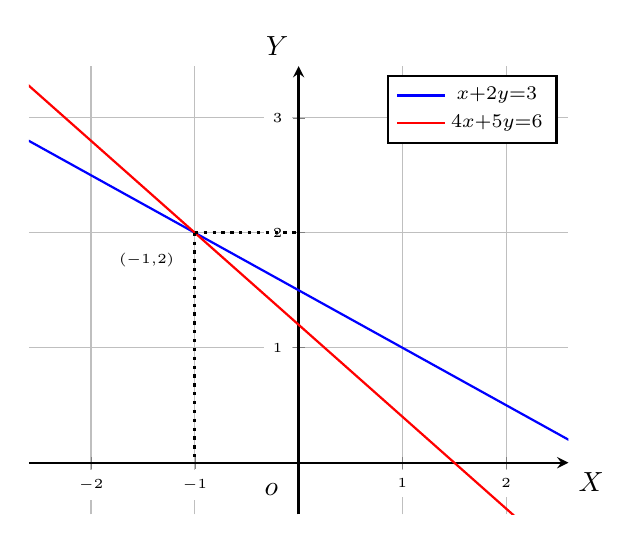
\begin{tikzpicture}
  \begin{axis}[standard,
      xtick={-2,-1,0,1,2},
      ytick={0,1,2,3,4,5},
      xticklabels={$-2$,$-1$,$0$,$1$,$2$},
      yticklabels={$0$,$1$,$2$,$3$,$4$,$5$},
      xlabel=$X$,
      ylabel=$Y$,
      samples=1000,
      xmin=-2,xmax=2,
      ymin=0,ymax=3,
      legend entries={${\scriptstyle x + 2y = 3}$,${\scriptstyle 4x + 5y = 6}$},
      grid=both,
    ]
    \node[anchor=center,label=south west:$o$] at (axis cs:0,0){};
    \node[anchor=center,label=south west:{${\scriptscriptstyle(-1,2)}$}] at (axis cs:-1,2){};
    \addplot[blue] {1.5 - (x/2)};
    \addplot[red] {6/5 - 4/5*x};
    \addplot[black,very thick,dotted] coordinates {
      (-1,2) (-1,0)

      (-1,2) (0,2)
    };
  \end{axis}
\end{tikzpicture}
\caption{\textbf{Set 1:} We can see that the 2 equations $x+2y=3$ and $4x+5y=6$
intersect at $(-1,2)$. Since they intersect at exactly one point and diverge before and after it, we can deduce that this system of equations has exactly one (i.e., unique) solution.
}
\end{figure}

\begin{figure}
  \centering
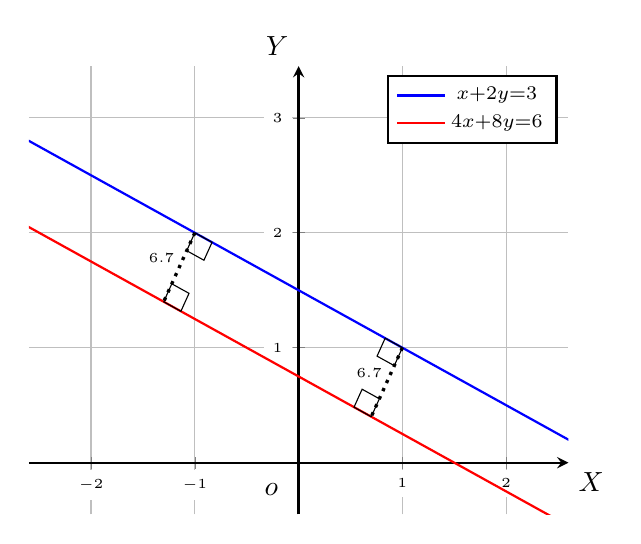
\begin{tikzpicture}
  \begin{axis}[standard,
      xtick={-2,-1,0,1,2},
      ytick={0,1,2,3,4,5},
      xticklabels={$-2$,$-1$,$0$,$1$,$2$},
      yticklabels={$0$,$1$,$2$,$3$,$4$,$5$},
      xlabel=$X$,
      ylabel=$Y$,
      samples=1000,
      xmin=-2,xmax=2,
      ymin=0,ymax=3,
      legend entries={${\scriptstyle x + 2y = 3}$,${\scriptstyle 4x + 8y = 6}$},
      grid=both,
    ]
    \node[anchor=center,label=south west:$o$] at (axis cs:0,0){};
    \node[anchor=center,label=south west:${\scriptscriptstyle 6.7}$] at (axis cs:-1,2){};
    \node[anchor=center,label=south west:${\scriptscriptstyle 6.7}$] at (axis cs:1,1){};
    \coordinate (A) at (axis cs:1,1){};
    \coordinate (B) at (axis cs:-1,2){};
    \coordinate (C) at (axis cs:0.7,0.4){};
    \coordinate (D) at (axis cs:-1.3,1.4){};
    \addplot[blue,name path=f] {1.5 - (x/2)};
    \addplot[red,name path=s] {6/8 - 4/8*x};

    \addplot[black,very thick,dotted,name path=p1] coordinates {(-1,2) (-1.3,1.4)};
    \addplot[black,very thick,dotted,name path=p2] coordinates {(1,1) (0.7,0.4)};
  \end{axis}
  \tkzMarkRightAngle(B,A,C);
  \tkzMarkRightAngle(A,B,D);
  \tkzMarkRightAngle(A,C,D);
  \tkzMarkRightAngle(B,D,C);
\end{tikzpicture}
\caption{\textbf{Set 2:} We can see that the 2 equations $x+2y=3$ and $4x+8y=6$
are always equi-distant to each other (i.e., they are parallel). Hence we can deduce that this system of equations has no solution.}
\end{figure}

\begin{figure}
  \centering
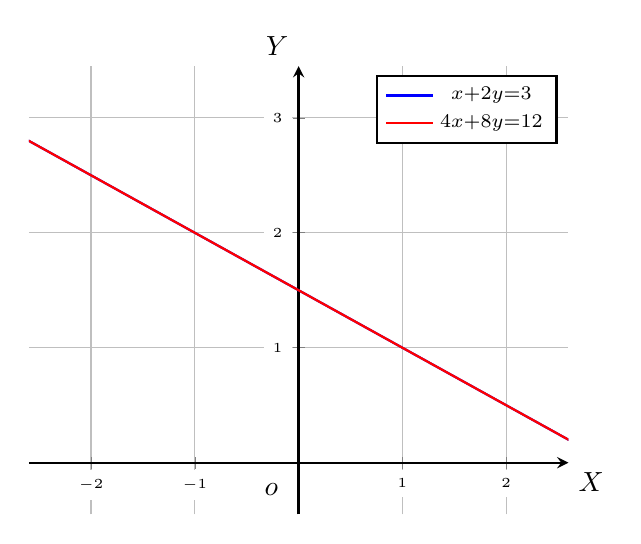
\begin{tikzpicture}
  \begin{axis}[standard,
      xtick={-2,-1,0,1,2},
      ytick={0,1,2,3,4,5},
      xticklabels={$-2$,$-1$,$0$,$1$,$2$},
      yticklabels={$0$,$1$,$2$,$3$,$4$,$5$},
      xlabel=$X$,
      ylabel=$Y$,
      samples=1000,
      xmin=-2,xmax=2,
      ymin=0,ymax=3,
      legend entries={${\scriptstyle x + 2y = 3}$,${\scriptstyle 4x + 8y = 12}$},
      grid=both,
    ]
    \node[anchor=center,label=south west:$o$] at (axis cs:0,0){};
    \addplot[blue] {1.5 - (x/2)};
    \addplot[red] {12/8 - 4/8*x};
  \end{axis}
\end{tikzpicture}
\caption{\textbf{Set 3:} We can see that the 2 equations $x+2y=3$ and $4x+8y=12$
coincide. Hence wee can deduce that this system of equations has infinite solutions (i.e., all the points on the lines).}
\end{figure}

%% -------------------------------- Problem #4.b -----------------------------------------------
\subparagraph{(b)}

\begin{itemize}
\item Set 1 
  \[\begin{split}
  &x + 2y = 3, 4x + 5y = 6\\
  \implies &x = 3 - 2y \implies 4(3-2y) + 5y = 6\\
  \implies &y = 2\text{ and }x = -1\\
  \implies &\boxed{\text{Unique Solution}}
  \end{split} \]
  Algebraically we see that only one pair of (x,y) satisfies both equations which gives us an unique solution. The observation matches with what we deduced from the graph of the equations.
\item Set 2 
  \[\begin{split}
  &x + 2y = 3, 4x + 8y = 6\\
  \implies &x = 3 - 2y \implies 4(3-2y) + 8y = 6\\
  \implies &12 -8y +8y = 6\text{ but }12 \not = 6\\
  \implies &\boxed{\text{No Solution}}
  \end{split} \]
  We can see that there is no solution for this system of equations as they both have the same slope but different intercepts. The observation is same as what we find from the graphical solution.
\item Set 3 
  \[\begin{split}
  &x + 2y = 3, 4x + 8y = 12\\
  \implies &x = 3 - 2y \implies 4(3-2y) + 8y = 12\\
  \implies &12 -8y +8y = 12\text{ but }12 = 12\\
  \implies &\text{Any (x,y) satisfying x + 2y = 3 is a Solution}\\
  \implies &\boxed{\text{Infinite Solutions}}
  \end{split} \]
  We can see that by multiplying with 4 on both sides to the first equation, we get the second equation. Hence algebraically both equations are the same. From the graph we saw that both the equations concide which is the same as what we observe algebraically.
\end{itemize}

%% -------------------------------- Problem #4.c -----------------------------------------------
\subparagraph{(c)}

\begin{itemize}
\item Set 1: $x + 2y = 3, 4x + 5y = 6$ in $\mathbf{Ax} = \mathbf{b}$ format can be expressed as
\[\begin{split}
  \begin{pmatrix}1&2\\4&5\end{pmatrix} \begin{pmatrix}x\\y\end{pmatrix}
  = \begin{pmatrix}3\\6\end{pmatrix}
  \implies x\begin{pmatrix}1\\4\end{pmatrix} + y \begin{pmatrix}2\\5\end{pmatrix}
  = \begin{pmatrix}3\\6\end{pmatrix}
\end{split}\]
We can see that $(1,4)$ and $(2,5)$ are linearly independent and all linear combinations of them span $\mathbb{R}^2$ (i.e,. they form the basis of $\mathbb{R}^2$). Hence any vector in $\mathbb{R}^2$ can be expressed as a linear combination of the 2 vectors with unique coefficients (i.e., unique solution).
\item Set 2: $x + 2y = 3, 4x + 8y = 6$ in $\mathbf{Ax} = \mathbf{b}$ format can be expressed as
\[\begin{split}
  \begin{pmatrix}1&2\\4&8\end{pmatrix} \begin{pmatrix}x\\y\end{pmatrix}
  = \begin{pmatrix}3\\6\end{pmatrix}
  \implies x\begin{pmatrix}1\\4\end{pmatrix} + y \begin{pmatrix}2\\8\end{pmatrix}
  = \begin{pmatrix}3\\6\end{pmatrix}
\end{split}\]
We can see that $(1,4)$ and $(2,8)$ are linearly dependent. Hence all linear combinations of them don't span $\mathbb{R}^2$. Hence only the vector which is a scalar multiple of them can be expressed as a linear combination of them with non-unique coefficients (i.e., no solution or infinite solutions). But since the vector $(3,6)$ is not a scalar multiple, this has no solution.
\item Set 3: $x + 2y = 3, 4x + 8y = 12$ in $\mathbf{Ax} = \mathbf{b}$ format can be expressed as
\[\begin{split}
  \begin{pmatrix}1&2\\4&8\end{pmatrix} \begin{pmatrix}x\\y\end{pmatrix}
  = \begin{pmatrix}3\\12\end{pmatrix}
  \implies x\begin{pmatrix}1\\4\end{pmatrix} + y \begin{pmatrix}2\\8\end{pmatrix}
  = \begin{pmatrix}3\\12\end{pmatrix}
\end{split}\]
We can see that $(1,4)$ and $(2,8)$ are linearly dependent. Hence all linear combinations of them don't span $\mathbb{R}^2$. Hence only the vector which is a scalar multiple of them can be expressed as a linear combination of them with non-unique coefficients (i.e., no solution or infinite solutions). But since the vector $(3,12)$ is a scalar multiple, this has infinite solutions.
\end{itemize}

%% -------------------------------- Problem #5 -----------------------------------------------
\pagebreak
\paragraph{5.} Review of Matrices:
\[
\mathbf{a} = \begin{pmatrix} -209/362\\-209/362\\209/362 \end{pmatrix},
\mathbf{b} = \begin{pmatrix} 0\\-408/577\\-408/577 \end{pmatrix},
\mathbf{c} = \begin{pmatrix} 396/485\\-198/485\\198/485 \end{pmatrix}
\]

%% -------------------------------- Problem #5.a -----------------------------------------------
\subparagraph{(a)} Given that,
\begin{equation}
\label{5a}
\mathbf{a.b} = \sum_{i=1}^n a_ib_i\text{ where }\mathbf{a,b}\in\mathbb{R}^n
\end{equation}

From equation \ref{5a}
\[\begin{split}
  \mathbf{a.b} &= \begin{pmatrix} -209/362\\-209/362\\209/362 \end{pmatrix} 
                .\begin{pmatrix} 0\\-408/577\\-408/577 \end{pmatrix}\\
  &= 0 + \left(\frac{209\times408}{362\times577}\right) - \left(\frac{209\times408}{362\times577}\right)\\
  &= 0\\
  \mathbf{a.c} &= \begin{pmatrix} -209/362\\-209/362\\209/362 \end{pmatrix} 
                .\begin{pmatrix} 396/485\\-198/485\\198/485 \end{pmatrix}\\
  &= -\left(\frac{209\times396}{362\times485}\right)
  + \left(\frac{209\times198}{362\times485}\right)
  + \left(\frac{209\times198}{362\times485}\right)\\
  &= 0\\
  \mathbf{b.c} &= \begin{pmatrix} 0\\-408/577\\-408/577 \end{pmatrix} 
                .\begin{pmatrix} 396/485\\-198/485\\198/485 \end{pmatrix}\\
  &= 0 + \left(\frac{408\times198}{577\times485}\right) - \left(\frac{408\times198}{577\times485}\right)\\
  &= 0\\
  \implies &\boxed{\mathbf{a.b} = \mathbf{a.c} = \mathbf{b.c} = 0}
\end{split} \]
%% -------------------------------- Problem #5.b -----------------------------------------------

\subparagraph{(b)}
Given that,
\begin{equation}
\label{5b}
\text{geometric length of a vector }\mathbf{a} = \sqrt{\mathbf{a.a}}\text{ where }\mathbf{a}\in\mathbb{R}^n
\end{equation}

From equation \ref{5b}
\[\begin{split}
  \text{geometric length of a vector }\mathbf{a}
  &= \sqrt{\begin{pmatrix} -209/362\\-209/362\\209/362 \end{pmatrix}
  .\begin{pmatrix} -209/362\\-209/362\\209/362 \end{pmatrix}}\\
  &= \sqrt{\left(\frac{209}{362}\right)^2 + \left(\frac{209}{362}\right)^2 + \left(\frac{209}{362}\right)^2}\\
  &= \left(\frac{209}{362}\right)\sqrt{3} \approx 1\\
  \implies &\boxed{\text{geometric length of }\mathbf{a} = 1}\\
\end{split} \]
\[\begin{split}
  \text{geometric length of a vector }\mathbf{b}
  &= \sqrt{\begin{pmatrix} 0\\-408/577\\-408/577 \end{pmatrix}
  .\begin{pmatrix} 0\\-408/577\\-408/577 \end{pmatrix}}\\
  &= \sqrt{0 + \left(\frac{408}{577}\right)^2 + \left(\frac{408}{577}\right)^2}\\
  &= \left(\frac{408}{577}\right)\sqrt{2} \approx 1\\
  \implies &\boxed{\text{geometric length of }\mathbf{b} = 1}\\
\end{split} \]
\[\begin{split}
  \text{geometric length of a vector }\mathbf{c}
  &= \sqrt{\begin{pmatrix} 396/485\\-198/485\\198/485 \end{pmatrix}
  .\begin{pmatrix} 396/485\\-198/485\\198/485 \end{pmatrix}}\\
  &= \sqrt{\left(\frac{396}{485}\right)^2 + \left(\frac{198}{485}\right)^2 + \left(\frac{198}{485}\right)^2}\\
  &= \left(\frac{198}{485}\right)\sqrt{6} \approx 1\\
  \implies &\boxed{\text{geometric length of }\mathbf{c} = 1}\\
\end{split} \]
\[\begin{split}
  \text{geometric length of a vector }\mathbf{x}
  &= \sqrt{\begin{pmatrix} 2\\-40/57\\8/77 \end{pmatrix}
  .\begin{pmatrix} 2\\-40/57\\8/77 \end{pmatrix}}\\
  &= \sqrt{\left(2\right)^2 + \left(\frac{40}{57}\right)^2 + \left(\frac{8}{77}\right)^2}\\
  &= \sqrt{4 + 0.4925 + 0.0108} = 2.1221\\
  \implies &\boxed{\text{geometric length of }\mathbf{x} = 2.1221}\\
\end{split} \]

%% -------------------------------- Problem #5.c -----------------------------------------------
\subparagraph{(c)}

\[
\begin{split}
\mathbf{A} &= \begin{pmatrix}
  -209/362 &0 &396/485\\
  -209/362 &-408/577 &-198/485\\
  209/362 &-408/577 &198/485
\end{pmatrix}\\
\implies \mathbf{Ax} &= \begin{pmatrix}
  -209/362 &0 &396/485\\
  -209/362 &-408/577 &-198/485\\
  209/362 &-408/577 &198/485
\end{pmatrix}
\begin{pmatrix} 2\\-40/57\\8/77 \end{pmatrix}\\
&= \begin{pmatrix} -1.0699\\ -0.7009\\ 1.6933 \end{pmatrix}\\
\implies \text{geometric length of }\mathbf{Ax}
&= \sqrt{\begin{pmatrix} -1.0699\\ -0.7009\\ 1.6933 \end{pmatrix}
  .\begin{pmatrix} -1.0699\\ -0.7009\\ 1.6933 \end{pmatrix}} = 2.122\\
\implies \text{geometric length of }\mathbf{Ax} &= \text{geometric length of }\mathbf{x}
\end{split}
\]
\boxed{\therefore\text{We observe that the geometric length of $\mathbf{x}$ is same as that of $\mathbf{Ax}$}}

%% -------------------------------- Problem #5.d -----------------------------------------------
\subparagraph{(d)}

\[
\begin{split}
\mathbf{A} &= \begin{pmatrix}
  -209/362 &0 &396/485\\
  -209/362 &-408/577 &-198/485\\
  209/362 &-408/577 &198/485
\end{pmatrix}\\
\mathbf{A}^T &= \begin{pmatrix}
  -209/362 &-209/362 &209/362\\
  0 &-408/577 &-408/577\\
  396/485 &-198/485 &198/485
\end{pmatrix}\\
\implies \mathbf{A}^T\mathbf{A} &=
\begin{pmatrix}
  -209/362 &0 &396/485\\
  -209/362 &-408/577 &-198/485\\
  209/362 &-408/577 &198/485
\end{pmatrix}
\begin{pmatrix}
  -209/362 &-209/362 &209/362\\
  0 &-408/577 &-408/577\\
  396/485 &-198/485 &198/485
\end{pmatrix}\\
&\approx \begin{pmatrix}
1 &0 &0\\
0 &1 &0\\
0 &0 &1
\end{pmatrix}\\
\implies \mathbf{A}\mathbf{A}^T &=
\begin{pmatrix}
  -209/362 &-209/362 &209/362\\
  0 &-408/577 &-408/577\\
  396/485 &-198/485 &198/485
\end{pmatrix}
\begin{pmatrix}
  -209/362 &0 &396/485\\
  -209/362 &-408/577 &-198/485\\
  209/362 &-408/577 &198/485
\end{pmatrix}\\
&= \begin{pmatrix}
3(209/362)^2 &0 &0\\
0 &2(408/577)^2 &0\\
0 &0 &6(198/485)^2
\end{pmatrix}
\approx \begin{pmatrix} 1 &0 &0\\ 0 &1 &0\\ 0 &0 &1 \end{pmatrix}\\
\end{split}
\]
\[\boxed{
\therefore
\mathbf{A}\mathbf{A}^T =
\begin{pmatrix}
1 &0 &0\\
0 &1 &0\\
0 &0 &1
\end{pmatrix},\,
\mathbf{A}^T\mathbf{A} =
\begin{pmatrix}
1 &0 &0\\
0 &1 &0\\
0 &0 &1
\end{pmatrix}\\
}\]

%% -------------------------------- Problem #5.e -----------------------------------------------
\subparagraph{(e)} Given that,
\begin{equation}\label{5e}\begin{split}
&\mathbf{AA}^T = \mathbf{I}\text{, where }\mathbf{A}\text{ is a full rank matrix}\\
\implies &\mathbf{A}^{-1}\mathbf{AA}^T = \mathbf{A}^{-1}I\\
\implies &\mathbf{A}^T = \mathbf{A}^{-1}\\
\implies &\mathbf{A}^T\mathbf{A} = \mathbf{A}^{-1}\mathbf{A} = I\\
\implies &\boxed{\mathbf{AA}^T = \mathbf{A}^T\mathbf{A} = \mathbf{I}}
\end{split}\end{equation}\\

We know that geometric length of a vector $\mathbf{v} = \begin{pmatrix} x\\y\\z \end{pmatrix},\,x,y,z\in\mathbb{R}$ is
$\,\sqrt{\mathbf{v}.\mathbf{v}}\,$ i.e., $\,\sqrt{x^2 + y^2 + z^2}$\\
which can be written as $\sqrt{\mathbf{v}^T\mathbf{v}}$, as

\begin{equation}\label{5e1}\begin{split}
\mathbf{v}^T\mathbf{v} &= \begin{pmatrix}x&y&z\end{pmatrix}\begin{pmatrix}x\\y\\z\end{pmatrix}
    = \begin{pmatrix}x^2 + y^2 + z^2\end{pmatrix}\\
\implies &\boxed{\text{geometric length of a vector} = \sqrt{\mathbf{v}^T\mathbf{v}}}
\end{split}\end{equation}

Let $\mathbf{v}_1 = \begin{pmatrix} a_1\\b_1\\c_1 \end{pmatrix}$ and
$\mathbf{v}_2 = \begin{pmatrix} a_2\\b_2\\c_2 \end{pmatrix}$, then
\begin{equation}\label{5e2}\begin{split}
    &(\mathbf{v}_1 + \mathbf{v}_2)^T = \begin{pmatrix} a_1 + a_2\\b_1 + b_2\\c_1 + c_2 \end{pmatrix}^T
    = \begin{pmatrix} a_1 + a_2&b_1 + b_2&c_1 + c_2 \end{pmatrix}\\
    &\mathbf{v}_1^T + \mathbf{v}_2^T = \begin{pmatrix}a_1&b_1&c_1\end{pmatrix}
      + \begin{pmatrix}a_2&b_2&c_2\end{pmatrix}
      = \begin{pmatrix} a_1 + a_2&b_1 + b_2&c_1 + c_2 \end{pmatrix}\\
    \implies &\boxed{(\mathbf{v}_1 + \mathbf{v}_2)^T = \mathbf{v}_1^T + \mathbf{v}_2^T}
\end{split}\end{equation}\\

We know that,
\begin{equation}\label{5e3}\begin{split}
  \mathbf{Av} &= x\begin{pmatrix}a\\d\\g\end{pmatrix}
  + y\begin{pmatrix}b\\e\\h\end{pmatrix}
  + z\begin{pmatrix}c\\f\\i\end{pmatrix}
  \text{, where }\mathbf{A} = \begin{pmatrix} a&b&c\\d&e&f\\g&h&i \end{pmatrix}\\
  \implies (\mathbf{Av})^T &= x\begin{pmatrix}a\\d\\g\end{pmatrix}^T
  + y\begin{pmatrix}b\\e\\h\end{pmatrix}^T
  + z\begin{pmatrix}c\\f\\i\end{pmatrix}^T\,\,[\text{from equation \ref{5e2}}]\\
  &= x\begin{pmatrix}a&d&g\end{pmatrix}
  + y\begin{pmatrix}b&e&h\end{pmatrix}
  + z\begin{pmatrix}c&f&i\end{pmatrix}\\
  &= \begin{pmatrix} x&y&z \end{pmatrix}\begin{pmatrix} a&d&g\\b&e&h\\c&f&i \end{pmatrix}\\
  \implies &\boxed{(\mathbf{Av})^T =\mathbf{v}^T\mathbf{A}^T}
\end{split}\end{equation}

$\therefore$ From equations \ref{5e1} and \ref{5e3}, geometric length of $\mathbf{Av}$ is
\[\begin{split}
\sqrt{(\mathbf{Av}).(\mathbf{Av})} &= \sqrt{(\mathbf{Av})^T\mathbf{Av}}
\text{, where }\mathbf{v} = \begin{pmatrix}x\\y\\z\end{pmatrix}\\
  &= \sqrt{\mathbf{v}^T\mathbf{A}^T\mathbf{Av}}
  = \sqrt{\mathbf{v}^T(\mathbf{A}^T\mathbf{A})\mathbf{v}}\\
  &= \sqrt{\mathbf{v}^T(\mathbf{I})\mathbf{v}}\,\,\,\,[\text{from equation \ref{5e}}]\\
  &= \sqrt{\mathbf{v}^T\mathbf{v}} = \sqrt{\mathbf{v}.\mathbf{v}}\\
  &= \text{geometric length of }\mathbf{v}\\
  \text{geometric length of }\mathbf{Av} &= \text{geometric length of }\mathbf{v}
\end{split}\]

\[\boxed{\text{Hence observation in part(c) will always be true for any $\mathbf{x}$, given equation \ref{5e}}}\]

\end{document}


%% Local Variables:
%% eval: (async-shell-command "zathura out/0.pdf &")
%% eval: (async-shell-command "latexmk -output-directory=out -pdf -pvc -interaction=nonstopmode 0.tex &")
%% End:
